\chapter{Preliminary Results}
\label{chap:prelim}

\section{SAT-like Hamiltonian}
\begin{figure}[h]
	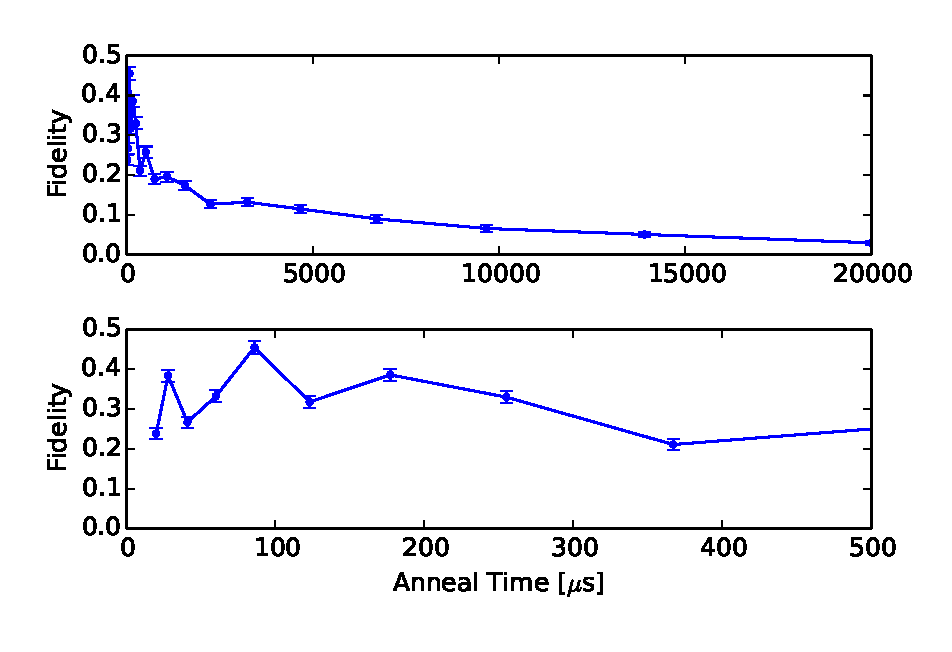
\includegraphics{img/6_018_2_fidelity.eps}
	\caption[Fidelity vs Time]{Plot of the fidelity as a function of annealing time for the Hamiltonian ``6\_018'' for both the full time range and the first 10 time points.  Both windows show the same data set.  Errors are estimated from $\sigma = \sqrt{np(1-p)}$.  Interesting features include the decrease in fidelity with longer anneal time and that the fidelity is very volatile over the short anneal time periods.}
	\label{fig:fidelity}
\end{figure}

Preliminary results were gathered on a sample quasi-random Hamiltonian called ``6\_018''.  This problem Hamiltonian was built up of clusters of clause sub-Hamiltonians in the same way as a SAT solver Hamiltonian would be, although ``6\_018'' does not encode a actual SAT problem.  This Hamiltonian was simple to generate and allowed us to verify our procedure for analyzing AQC results.
Data was collected in a series of evolutions at annealing times ranging from 20 $\mu$s to 20 ms.  Each evolution consists of choosing an anneal time and programming the problem Hamiltonian onto the hardware, then annealing 1000 times successively and reading out the final states.  We call each of these individual evaluations a \emph{read}, and a whole sequence of reads with the same programmed Hamiltonian a \emph{run}.  Any programming error (see \ref{sec:noise}) in the Hamiltonian should be the same between reads and differ between runs.

The state read out after each read is either the ground state, or some other higher energy (and incorrect) state.  The successes and failures thus follow a binomial distribution; there is some probability $p$ of getting the ground state, and probability $1-p$ of getting a different state.
Our best estimate of the fidelity from a single run is thus the fraction of successes, or $p = \frac{gs}{n}$ for $gs$ reads of the ground state and $n$ total reads.  We can also estimate the error in our estimate of the fidelity, because the variance of a binomial distribution is $\sigma^2 = np(1-p)$.

Figure \ref{fig:fidelity} shows the results of an initial set of runs spanning annealing times from 20 $\mu$s to 20 ms.  
There are several features of this data that stand out.  
First, contrary to our expectations, the fidelity \emph{decreases} as the anneal time increases.  We would expect that longer anneal times bring us closer to adiabatic evolution and thus remaining in the ground state.  This result suggests to us that adiabaticity (or lack thereof) is not dominating the fidelity for long annealing times. 
Second, there is significant change in the fidelity over very small changes in anneal time for less than $\sim 300$ $\mu$s, well outside what we would statistically expect based on the number of reads conducted.  This suggests that there is an uncontrolled factor besides the annealing time when the anneal time is short.  This factor disappears for longer anneal times, when whatever is damping the fidelity also seems to dampen the short time oscillations.

Figure \ref{fig:short_fidelity} shows the same data as in Figure \ref{fig:fidelity} as well as three more sweeps conducted in the same fashion, annealing out to 500 $\mu$s.  The large-short time oscillations are still seen, and of note is the fact that different runs of the same anneal time lie far outside their respective error margins.  This confirms our earlier suspicion that rather than the quantum annealing fidelity actually changing so rapidly with small changes in anneal time, there is some other uncontrolled factor which is changing from run to run.

\begin{figure}
	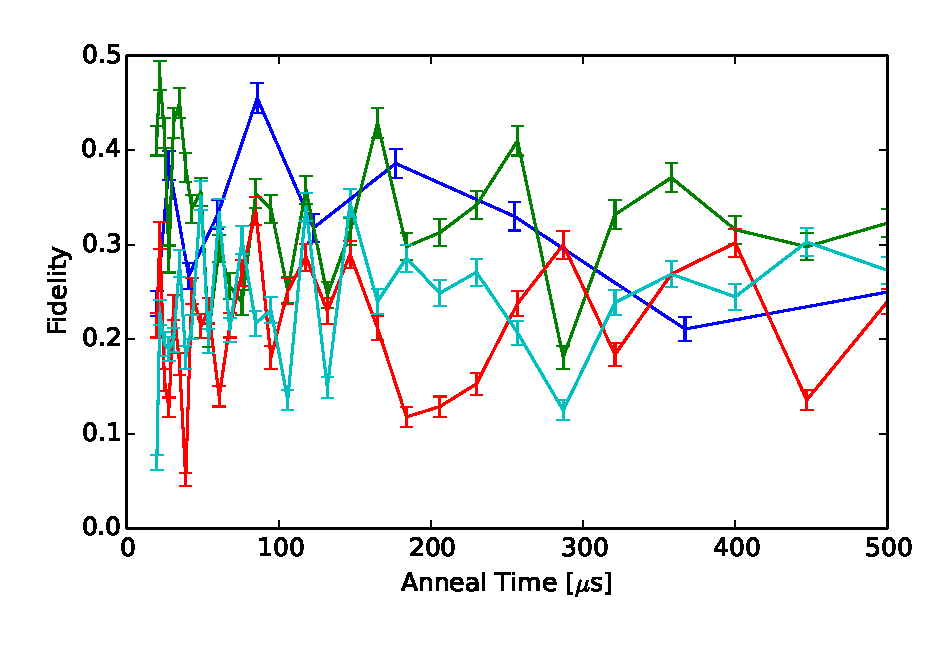
\includegraphics{img/6_018_comparison.eps}
	\caption[Short Time Fidelities]{The fidelity as a function of time for the Hamiltonian ``6\_018'' for several different machine runs.  Each data point consist of 1000 machine reads.  Notice the spread between machine runs is outside of the error bars.}
	\label{fig:short_fidelity}
\end{figure}

\section{Single Qubyte Hamiltonian}
The Hamiltonian shown in the above figures is large and reasonably complicated, with blocks of clauses and chains of clone spins spread across many qubytes.  Simplifying the Hamiltonian until we see smooth fidelity vs. time curves as we expect, and then increasing the complicating factors until we see the oscillations emerge would let us figure out what's causing them.  To that end a simple Hamiltonian ``k44'' consisting of a single qubyte of spins and encoding the logic of a single SAT clause was evaluated in the same fashion as the earlier ``6\_018'': runs at anneal times from 20 $\mu$s to 500 $\mu$s with 1000 reads per run.  

Figure \ref{fig:k44_comparison} shows the results of two such sweeps.  While the fidelity is higher than in the larger Hamiltonian's case, the short-time oscillations are still present.  The fidelity increase is in line with our expectations; as the number of spins grows the gap shrinks and fidelity drops for a given anneal time.  The continued presence of the short-time oscillations indicates that they're not simply a result of ``difficulty'' of the Hamiltonian (i.e. the gap or the problem size), but some other factor.

\begin{table}
	\begin{center}
\begin{tabular}{ | l | l | l | l |}
	\hline
	\multicolumn{4}{|c|}{k44 Hamiltonian} \\ \hline
	\multicolumn{2}{|c|}{Fields} & \multicolumn{2}{c|}{Couplings} \\ \hline
	A & 1.0 & A,B & 1.0 \\
	B & 1.0 & A,D & -2.0 \\
	C & -1.0 & B,D & -2.0 \\
	D & -3.0 & C,D & 1.0 \\ \hline
\end{tabular}
\end{center}
\caption[k44 Hamiltonian]{The fields and couplings making up the Hamiltonian ``k44''.}
\end{table}

\begin{figure}
	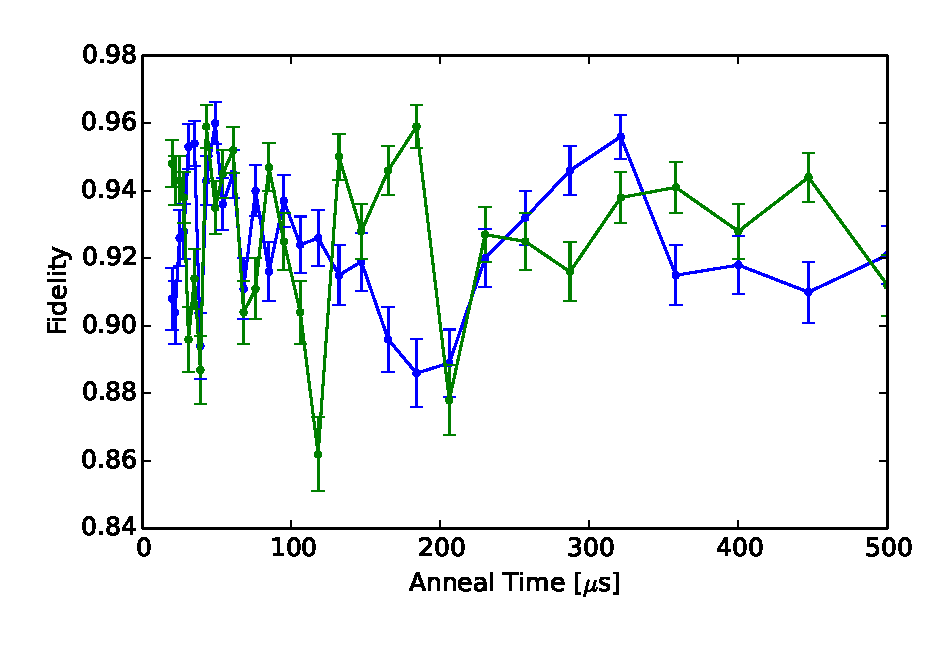
\includegraphics{img/k44.eps}
	\caption[Single K44 Fidelity]{Fidelity as a function of anneal time for the Hamiltonian ``k44'' which consists of a single SAT clause embedded into a single qubyte.  The fidelity is higher than ``6\_018'' for the same anneal times, but the short-time oscillations are still present.}
	\label{fig:k44_comparison}
\end{figure}

\section{Boolean SAT Hamiltonian}
The last preliminary investigation was conducted on a six variable, 21 clause 3-SAT Hamiltonian with two satisfying assignments, FIXME.  When embedded this Hamiltonian filled essentially the entire hardware graph.  Figure \ref{fig:test_6} shows the estimated fidelity from anneal times ranging from 20 $\mu$s to 500 $\mu$s, estimated from 1000 reads and single runs at each anneal time.  The fidelity is close to zero throughout the time range.  In contrast to our previously observed Hamiltonians, the \machine machine seems unable to successfully solve this particular problem instance.  

Figure \ref{fig:test_6_hist} is a pair of histograms showing all 1000 results of annealing at 20 $\mu$s for both the ``6\_018'' Hamiltonian and the 3-SAT Hamiltonian.  The peak of the distribution for ``6\_018'' is near the ground state, while the peak of the distribution for the 3-SAT Hamiltonian is in the neighbourhood of the 10th excited state.  Presumably this is due to the energy levels of the 3-SAT Hamiltonian closing together where the ``6\_018'' levels do not.  The distribution of the results for the 3-SAT Hamiltonian is also broader, for reasons which are not clear.  Both of these Hamiltonians are much to large to be simulated classically, so we cannot predict how the energy levels change over the annealing to explain the distribution differences directly.

\begin{figure}
	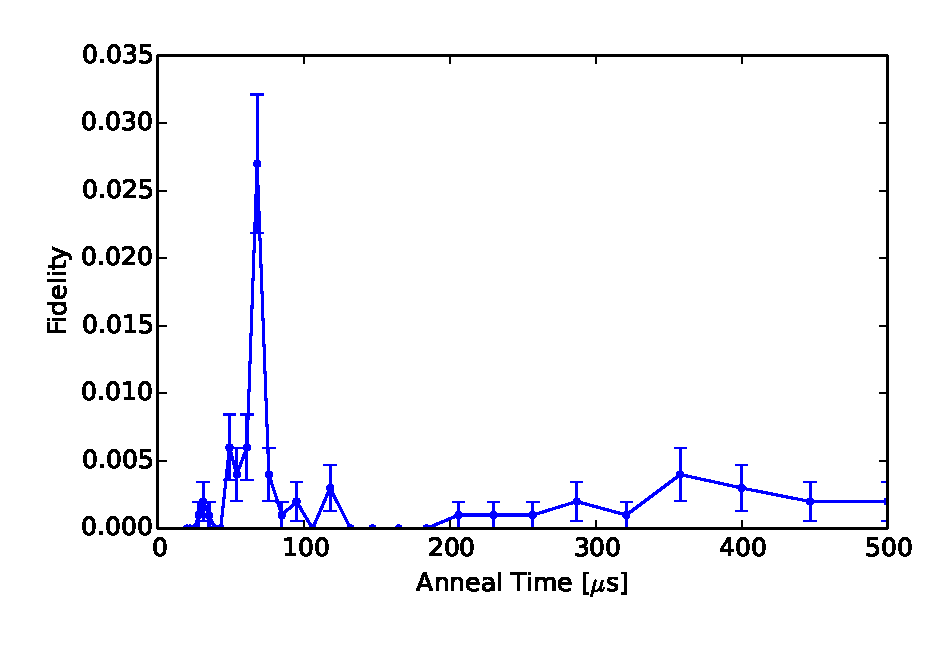
\includegraphics{img/test_6.eps}
	\caption[Result of a 6 Variable 3-SAT Instance]{This figure shows the estimated fidelity as a function of annealing time for a six variable, 21 clause 3-SAT instance.  The fidelity is essentially zero throughout the time range.}
	\label{fig:test_6}
\end{figure}

\begin{figure}
	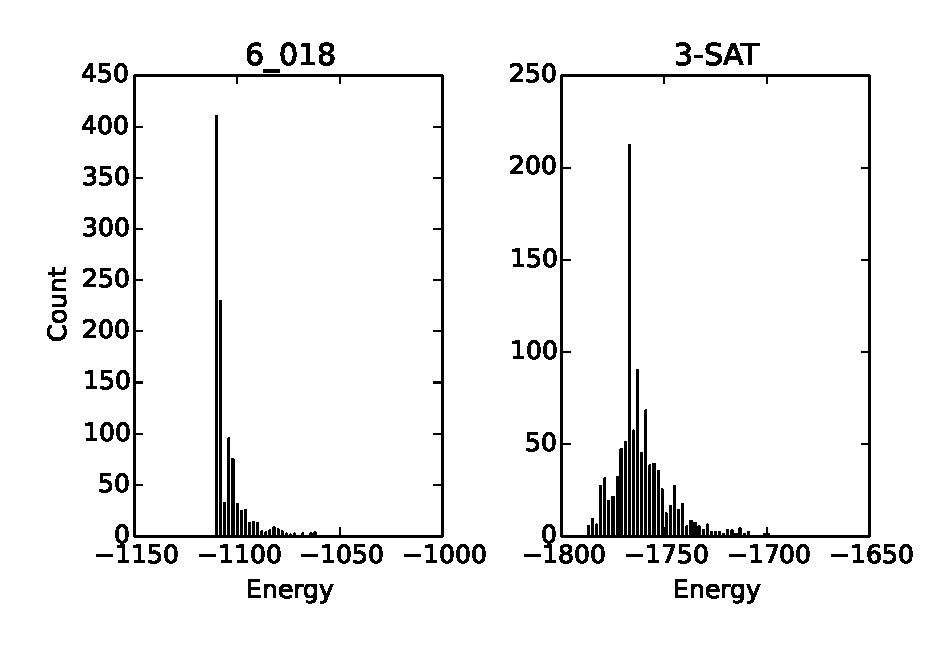
\includegraphics{img/hist.eps}
	\caption[20 $\mu$s Result State Histograms]{Histograms showing all 1000 states found after 20 $\mu$s of annealing for both ``6\_018'' on the left and the 6 variable 3-SAT on the right.  The fidelity is clearly much higher on the left.  While the distribution of the ``6\_018'' results peaks near the ground state and decays exponentially in a thermodynamic fashion, the 3-SAT results are peaked in the vicinity of the 10th excited state.}
	\label{fig:test_6_hist}
\end{figure}

Unfortunately there is not much we can do with such low fidelities, so the rest of the results will focus on simpler Hamiltonians such as ones which occupy single K44s.  This means we cannot benchmark the \machine machine to any degree as was the initial plan since actual 3-SAT problems, even those as small as 6 problem variables, are too difficult for the machine to solve reliably.

Having carried out these preliminary results, we have established a framework for evaluating the \machine machine: ascertain the cause of the large uncertainty in the short-time evolution results, using simpler Hamiltonians; measure the effect that number of spins has in a more fine grained manner; and check the intra-run results to see how much of an effect read noise has.
\begin{table}
	\begin{center}
\begin{tabular}{ | l | l | l | l |}
	\hline
	\multicolumn{4}{|c|}{k44\_and Hamiltonian} \\ \hline
	\multicolumn{2}{|c|}{Fields} & \multicolumn{2}{c|}{Couplings} \\ \hline
	A & 1.0 & A,B & 1.0 \\
	B & -1.0 & A,D & -2.0 \\
	C & 3.0 & B,D & -2.0 \\
	D & -1.0 & C,D & -1.0 \\ \hline
\end{tabular}
\end{center}
\caption[k44\_and Hamiltonian]{The fields and couplings that make up the Hamiltonian ``k44\_and''.  This single qubyte Hamiltonian has a single non-degenerate ground state: $\uparrow\uparrow\downarrow\uparrow$ }
\end{table}

The main Hamiltonian for the rest of the results will be ``k44\_and'', a single qubyte Hamiltonian similar to ``k44'' but featuring only a single non-degenerate ground state.
